\documentclass[letterpaper, 10 pt, conference]{ifacconf}  % Comment this line out
                                                          % if you need a4paper

\usepackage{graphicx}      % include this line if your document contains figures
\usepackage{natbib}        % required for bibliography. Does not work with ifac format together with hyperref package
%\usepackage{hyperref}
\usepackage{subfigure}
\usepackage{amsfonts}
\usepackage{amsmath}
\usepackage{amssymb}
\usepackage{makeidx}
\usepackage{epsfig}
%\usepackage{color}
%\usepackage[dvips]{color}
%\usepackage{amsthm}
\usepackage{makeidx,epsfig}
\usepackage{multirow}
\usepackage{mathrsfs}
%\usepackage[T1]{fontenc}          %%%%%% INSERIRE PER ACCENTO!!!!!!!!!!!!
%\usepackage[utf8]{inputenc}
%\usepackage[italian]{babel}
%\usepackage[table]{xcolor}
\usepackage{todonotes}
%\usepackage{menukeys}
\usepackage{algorithm,algpseudocode}
\usepackage{accents}
\usepackage{booktabs}

%\usepackage[font=small,justification=raggedright]{caption}
\newcommand\munderbar[1]{%
	\underaccent{\bar}{#1}}




\newcommand\todoin[2][]{\todo[inline, caption={2do}, #1]{
		\begin{minipage}{\textwidth-4pt}#2\end{minipage}}}
%\hypersetup{citecolor=black, colorlinks=false, linkcolor=black, pdfborder={0 0 0}}
\providecommand{\ad[1]}{{\color{blue}#1}}

%
%%===============================================================================
%
%\newtheorem{algorithm}{Algorithm}
%\newtheorem{assumption}{Assumption}
\newtheorem{theorem}{Theorem}
\newtheorem{corollary}[theorem]{Corollary}
\newtheorem{definition}{Definition}
\newtheorem{example}{Example}
\newtheorem{lemma}[theorem]{Lemma}
\newtheorem{proposition}[theorem]{Proposition}
\newtheorem{problem}{Problem}
\newtheorem{remark}{Remark}
\newtheorem{assumption}{Assumption}


%==============================================================================================================
%==============================================================================================================

\begin{document}

\begin{frontmatter}
	
	\title{Data-driven Switched Affine Modeling for Model Predictive Control\thanksref{footnoteinfo}} 
	% Title, preferably not more than 10 words.
	
	\thanks[footnoteinfo]{This work was supported by project \emph{INnovating City Planning through Information and Communication Technologies} (INCIPICT), and by TerraSwarm, one of six centers of STARnet, a Semiconductor Research Corporation program sponsored by MARCO and DARPA, and by the Italian Government under Cipe resolution n.135 (Dec. 21, 2012).}
	
	\author[First,Second]{Francesco Smarra} 
	\author[Second]{Achin Jain} 
	\author[Second]{Rahul Mangharam}
	\author[First]{Alessandro D'Innocenzo}
	
	\address[First]{Department of Information Engineering, Computer Science and Mathematics, University of L'Aquila, Via Vetoio, Coppito, 67100 L'Aquila, Italy \\(e-mail: [francesco.smarra,alessandro.dinnocenzo]@univaq.it).}
	\address[Second]{Department of Electrical and Systems Engineering, University of Pennsylvania, 200 South 33rd Street, 19104 Philadelphia, PA, USA (e-mail: [achinj,rahulm]@seas.upenn.edu)}

\begin{abstract}
Model Predictive Control (MPC) is a well consolidated technique to design optimal control strategies, due to its ability to predict system’s behavior over a future horizon. The main drawback that has not allowed the widespread adoption of MPC for large scale systems, such as buildings and process control, is related to the difficulties (cost, time, and effort) associated with the identification of accurate dynamical models. In the last years, to overcome this problem, researchers' attention has been focused on methodologies that are able to build mathematical models that are data-driven, i.e. based only on historical data of the systems. However, data-driven models are not suitable for control because of non-physical models. Recently, a Data Predictive Control (DPC) strategy, which implements finite Receding Horizon Control (RHC) using control-oriented data-driven models based on regression trees and random forests, has been proposed in the literature for energy savings in buildings. The drawback of this approach is that the mathematical model is based on static input-output relations, thus there is no internal state evolution. The goal of this paper is to derive a state-space model using regression trees algorithm, hence bridging the gap between the efficiency of DPC and control system theory. Differently from DPC, this modeling framework allows to verify system properties defined in system theory, i.e. stability, structural properties, etc., and apply classical control methodologies, e.g. MPC, without any knowledge on the system model. To show the value of our new methodology, a comparison with DPC in his native case study, i.e. building automation, is provided. It is shown that the results obtained with such approach are closer to the optimum than DPC ones.
\end{abstract}

\begin{keyword}
	Data-driven modeling, data-driven predictive control, machine learning, switched systems, MPC.
\end{keyword}

\end{frontmatter}
%==============================================================================================================
%==============================================================================================================

\section{INTRODUCTION}\label{secIntro}
Predictive models have been extensively studied in the last years to design optimal control strategies to improve systems performance. In particular, due to its capability to use dynamical models to predict systems' trajectories, Model Predictive Control (MPC) have been widely used, as for example in energy systems \cite{MaTCST2015,OldewurtelEB2012,MaasoumyEB2014,IovineIFAC2017}, to guarantee a desired system behavior while optimizing a desired performance.

The drawback of MPC is that it requires accurate models for the prediction. In the case of complex systems, such as buildings, smart grids, etc., obtaining such models can be cost and time prohibitive \cite{SturzeneggerTCST2016}. To overcome this issue, a possibility is to use machine learning algorithms to learn models using only historical data available to the system. However, such models are not directly suitable for control.

In recent years, researchers' attention has been focused on this problem. Indeed different works, \cite{Macarulla2017,Afram2017,Ferreira2012} and others, used machine learning algorithms, in particular neural networks, for predictive control. Nevertheless, none of these works addressed the problem of including data-driven state model in the optimal predictive control loop, and hence did not allow to set up MPC-like optimal control problems.

To the best of authors' knowledge, such problem has been addressed for the first time in \cite{BehlAE2016}, where data-driven models, built using regression trees algorithms, have been developed to enable one-step closed-loop predictive control for the demand-response problem in buildings. This approach has been extended in \cite{JainACC2017,JainCDC2017}, where the authors proposed a regression trees and random forests-based Data Predictive Control (DPC) strategy, that implements finite Receding Horizon Control (RHC). More precisely, they built a regression tree (and similarly a random forest) for each step of the predictive horizon using only system's initial state and disturbance data, and assigned to each leaf of each tree an affine function depending only on system inputs. This model is then used to predict system's behavior at next step. They used this modeling framework to set up a RHC problem for temperature tracking in a room. They showed how DPC can achieve comparable performance with MPC, but without utilizing any physical modeling of the system. However, the main drawback of this approach is due to the fact that the models used are static. In particular, the authors associated to each step of the horizon an affine model that is independent from previous steps, i.e. the model does not have an internal state evolution, and the prediction at different steps of the horizon depends only on the initial state and disturbance forecast. It follows that system's properties, such as stability, structural properties, etc. cannot be studied, and that closed-loop control does not have working guarantees.

The main contribution of this paper is a new methodology with the aim of exploiting the advantages of all the aforementioned approaches. More precisely, we propose a model predictive control scheme, where the dynamical model is a Switched Affine (SA) data-driven model obtained using regression trees. We show that we can keep the efficiency of the regression trees-based data-driven models, while guaranteeing the presence of an internal state evolution. To show the validity of our approach, we provide a comparison in the DPC native case study, i.e. building automation, and show that we do not loose in performance. On the contrary, our approach shows improvements with respect to DPC.

The paper is organized as follows. In Section \ref{secDPC} we briefly recall the DPC approach. In Section \ref{secDataDrivenModeling}, as the main contribution of this paper, we create a switched affine LTI system given a set of data and setup a Model Predictive Control Problem with our model. In Section \ref{secCaseStudy} we provide a case study to compare performance of our approach with the DPC.

\textbf{\emph{Notation.}} We denote by $I$ and $\bold{0}$ respectively the identity matrix and a matrix with all the entries equal to $0$ of appropriate dimensions, by $det(A)$ the determinant of matrix $A$, and by $\biguplus$ the disjoint union.

\section{Data Predictive Control}\label{secDPC}
In this section we briefly recall the concept of DPC introduced in \cite{JainACC2017}. This will be useful to both better understand and compare the approach we want to propose. The idea behind DPC is to create a model of a system using machine learning algorithm (in our case regression trees) starting from his historical data and that can be used in a receding horizon control scheme. Typically, models created using machine learning algorithms are not directly suitable for control, and hence need to be modified. To this aim DPC consider \emph{separation of variables}.

\textbf{Separation of variables.} Let a dataset $(\mathcal{X},\mathcal{Y})$ with $s$ samples for each feature (variable) be given. For $k=1,2,\ldots,s$, $\mathcal{X}$ is the set of control inputs $u\in\mathbb{R}^m$, disturbances $d\in\mathbb{R}^r$ and state variable $x\in\mathbb{R}^n$, and $\mathcal{Y}\in\mathbb{R}^n$ is the set of response variables $y$, that in our case will represent the state evolution over the horizon, i.e. $x(k+1),\ldots,x(k+N)$ given the current time $k$. We partition the set $\mathcal{X}=\{\mathcal{X}_c,\mathcal{X}_d\}$ into the set $\mathcal{X}_c$ of data associated to the $m$ control variables (or manipulated features) and the set $\mathcal{X}_d$ of data associated to the $r+n$ disturbance and state variables (or non-manipulated features). Using separation of variables, the training process to grow a tree $\mathcal{T}$ is divided into two steps:
\begin{enumerate}
\item the trees are trained only on $\mathcal{X}_d$. It is important to note that besides external disturbances, $\mathcal{X}_d$ can also contain past terms of the output $\mathcal{Y}$, as for example the initial state of the system;
\item affine function models are fit in the leaves (or terminal nodes) of the trees as function of only $u$. 
\end{enumerate}

\begin{remark}
	If we did not consider separation of variables and used also input variables to grow the tree, as in the right side of Figure \ref{figSeparationVariables}, the resulting model would not be suitable for control. This is because, since $u$ is the variable we want to optimize, we do not have the input component to go through the tree and so we cannot find the the leaf and thus the model to make the prediction. For more details see \cite{JainACC2017}.
\end{remark}

This training process is illustrated in the left side of Figure \ref{figSeparationVariables}. 
To obtain a model that can be used in a RHC problem with prediction horizon $N$, this procedure is used to grow multiple trees $\mathcal{T}_1,\ldots,\mathcal{T}_N$. Each tree is used to predict system's behavior at one step of the horizon.
Let $\ell_{i_j} = \{s_1,\ldots,s_\epsilon\}$, $i_j=1,\ldots,p_j$, be the $i_j^{th}$ leaf of $\mathcal{T}_j,\ j = 1,\ldots,N$, containing samples $s_1,\ldots,s_\epsilon \in \mathcal{X}_d$. Then the leaves of $\mathcal{T}_j$ form a partition of $\mathcal{X}_d$:

\begin{align}\label{distSetPartition}
	\mathcal{X}_d=\biguplus_{i_j=1}^{p_j}{\ell_{i_j}}, \quad \left(\ell_{\alpha}\cap \ell_{\beta}=\varnothing,\,\forall \alpha\neq \beta \right).
\end{align}

\subsection{DPC-RT: DPC with Regression Trees}
Without any loss of generality we consider $n=1$, but the results can be extended to multiple states considering multiple trees. The idea is to predict output $y$ over an horizon of length $N$ given the state measurement and the disturbance forecast at the current step. Applying the separation of variables it is possible to build $N$ regression trees $\mathcal{T}_j,\ j=1,\ldots,N$, using CART algorithm (\cite{Breiman1984classification}) and associate to each leaf $i_j$ of each tree the following affine static model:

\small
\begin{equation}\label{eqAffineModel}
	y(k+j) = \beta_{i_j}[1\ u(k) \cdots u(k+j-1)]^\top,\ \forall i_j\in T_j,\,\forall j,
\end{equation}
\normalsize

with $\beta_{i_j}\in\mathbb{R}^{jm+1}$.

\begin{remark}
	This algorithm can be seen as a procedure similar to linerization. In particular, the trees "linearize", by partitioning the dataset, over the disturbance and state variables in $\mathcal{X}_d$, while the action of the input variables in $\mathcal{X}_c$ in each leaf is assumed to be linear.
\end{remark}

\begin{remark}
	This method belongs to the class of recursive partitioning algorithms: the seminal algorithm for learning regression trees is CART~\cite{Breiman1984classification}. An important feature is that regression trees are by design highly interpretable, which is a fundamental desirable quality in any predictive model.
\end{remark}
Once these models are created, at each instant $k$ we can find coefficients $\beta_{i_j}$, for $j=1,\ldots,N$, in run-time to solve the following RHC optimization problem
\begin{problem}\label{pbDPC}

\small
\begin{equation*}
\begin{aligned}
& \underset{u_k}{\text{minimize}} & &  \sum_{j=1}^{N} y_{k+j}^2 Q + u^\top_{k+j-1} R u_{k+j-1} +  \lambda\varepsilon_j  \\
& \text{subject to }            & &  y_{k+j}        =   \beta_{i_j} [1\ u_{k} \cdots u_{k+j-1} ]^\top                   \\
&                               & &  u_{k+j-1}     \in  \mathcal{U}                                                     \\
&                               & &  |y_{k+j}|     \leq \bar{y} + \varepsilon_j 										\\
&                               & &  \varepsilon_j \geq  0																\\
&                               & &  j              =    1,\ldots,N,            									    \\
\end{aligned}
\end{equation*}
\normalsize
\end{problem}

where slack variables $\varepsilon_j$ ensure recursive feasibility of the algorithm. This problem is solved as in classical MPC. At each time step the optimal $u^*_k,\ldots,u^*_{k+N-1}$ are computed and only the first one is applied as control input, i.e. $u(k) = u^*_k$.
\begin{figure}[t!]
	\begin{center}
		\includegraphics[width=15pc]{figures/dpc-sepvars.eps}
		\caption{Separation of variables. \textit{Step 1:} Tree $\mathcal{T}_1$ is trained only on the disturbances $X_d$ as the features. Tree $\mathcal{T}_2$ uses both the disturbances $X_d$ and the control variables $X_c$ for splitting and is thus not computationally suitable for control. \textit{Step 2:} In the leaf $\ell_{i_j}$ of trees $\mathcal{T}_j$, a linear regression model parametrized by $\beta_{i_j}$ is defined as a function only of the control variables.}\label{figSeparationVariables}
	\end{center}
\end{figure}

%==============================================================================================================
%==============================================================================================================

\section{DATA-DRIVEN PREDICTIVE MODEL}\label{secDataDrivenModeling}
DPC modeling framework, although simple, is characterized by a main issue: the models in the leaves are affine functions that create an input-output \emph{static} relation described in \eqref{eqAffineModel}. Moreover, the current state is used only to find the tree leaf to select the affine model to use at a certain step of the horizon. To have a good prediction accuracy, parameters $\beta_{i_j}$ are different for each step, also if they multiply the same input component. Therefore in Problem \ref{pbDPC}, system's evolution at each step is independent from the inputs applied in the previous steps. This means system's modeling does not consider an internal state. As a consequence, another problem is that the lack of an internal state does not allow to to verify or guarantee system's properties such as stability, structural properties, etc..

The scope of this paper is to address this issue providing a data-driven state-space modeling framework using regression trees. To this aim we leverage separation of variables and replace affine static models \eqref{eqAffineModel} in the leaves with LTI models, creating a switched affine system of the form

\begin{equation}\label{eqSwitchedSystemOriginal}
x(k+1) = A_{\sigma_k}x(k) + B_{\sigma_k}u(k) + f_{\sigma_k}.
\end{equation}

\noindent $\sigma_k: \mathbb{N} \rightarrow \{i_1,\ldots,i_N\}$ is an exogenous signal that drives the switching rule assigning to each instant $k$, of the predictive horizon, the matrices corresponding to the leaf $\ell_{i_j}$. We see in Section \ref{ssecMPC-SA} that this task is not trivial, since replacing the affine functions in \eqref{eqAffineModel} with LTI models is not enough to guarantee an internal state evolution, so we propose an extension of the state-space to overcome this problem. Before that, in Section \ref{ssecEstimation} we setup a least square optimization problem in order to estimate $A_{\sigma_k}$, $B_{\sigma_k}$, and $f_{\sigma_k}$ from $(\mathcal{X},\mathcal{Y})$ using regression trees. Finally, we setup an MPC problem that will be used in Section \ref{secCaseStudy} to show the performance of the proposed approach.

\subsection{Estimation}\label{ssecEstimation}
Let us consider a prediction horizon equal to $N$. We create $N$ trees $\mathcal{T}_j$, $j = 1,\ldots,N$, each one built using disturbance $d(k+j-\delta),\ldots,d(k + j)$ and the current state $x'(k)$ data from $\mathcal{X}_d$. To each leaf $\ell_{i_j}$ of each tree $\mathcal{T}_j$ we associate a LTI model of the form:
\begin{equation}\label{eqLTIleaves}
	x'(k+j) = A'_{i_j}x'(k) + \sum_{\alpha = 1}^{j}{B'_{i_j,\alpha}u(k+\alpha-1)} + f'_{i_j}
\end{equation}
where $A'_{i_j}$, $B'_{i_j,\alpha}$ and $f'_{i_j}$ are identified using the least square method defined in Problem \ref{pbLeastSquareProblem} below. To this aim we consider the experiments associated to the samples $s_1,\ldots,s_\epsilon$ in the leaf $\ell_{i_j}$ at time instants $k_1,\ldots,k_\epsilon$, and their past $\nu$ values. In particular, for each leaf $\ell_{i_j}$, let us define
\small
\begin{align}
\Lambda_{i_j} &= \left[\begin{array}{ccc}
						1               & \cdots & 1                    \\ 
						x'(k_1)         & \cdots & x'(k_\epsilon)       \\  
						\vdots          &        &     \vdots           \\
						x'(k_1 - \nu)   & \cdots & x'(k_\epsilon - \nu) \\
						u_1(k_1)        & \cdots & u_1(k_\epsilon)      \\
						\vdots          &        & \vdots               \\
						u_m(k_1)        & \cdots & u_m(k_\epsilon)      \\ 
						\vdots          &        & \vdots               \\ 
						u_1(k_1 + j)    & \cdots & u_1(k_\epsilon + j)  \\
						\vdots          &        & \vdots               \\
						u_m(k_1  +j)    & \cdots & u_m(k_\epsilon + j)  \\   
				 \end{array}\right]^\top
\xi_{i_j}      = \left[\begin{array}{c}
				 		f \\ a_1 \\ \vdots \\ a_\nu \\ b_{1,1} \\ \vdots  \\ b_{m,1} \\ \vdots \\ b_{1,j} \\ \vdots \\ b_{m,j}
				 \end{array}\right]\\
%\xi_{i_j} 	  &= \left[\begin{array}{ccccccccccc}
%						f'_{i_j} & a_1 & \cdots & a_\nu & b_{1,1} & \cdots & b_{m,1} & \cdots & b_{1,j} & \cdots & b_{m,j}
%				 \end{array}\right]^\top\\
\lambda_{i_j} &= \left[\begin{array}{ccc}
						x'(k_1 + j + 1) & \cdots & x'(k_\epsilon + j + 1)
				 \end{array}\right]^\top
\end{align}
\normalsize

We use this setup to formalize the following problem to estimate matrices in \eqref{eqLTIleaves}.

\begin{problem}\label{pbLeastSquareProblem}
\small
\begin{alignat}{2}
\nonumber & \underset{\xi_{i_j}}{\text{minimize}} & &  \parallel \Lambda_{i_j} \xi_{i_j}  - \lambda_{i_j} \parallel_2^2            \\
		  & \text{subject to }                    & &  \Gamma_{eq}    \, \xi_{i_j} = \gamma_{eq}\label{eqEqualityConstraints}      \\
		  &                                       & &  \Gamma_{diseq} \, \xi_{i_j} = \gamma_{diseq}\label{eqInequalityConstraints}
\end{alignat}
\normalsize
\end{problem}

where \eqref{eqEqualityConstraints} and \eqref{eqInequalityConstraints} are used to constraint elements in $\xi_{i_j}$ due to physical reason of the plant. For example we use them in Section \ref{secCaseStudy} to constrain elements of matrix $\bar B_{\sigma_k}^\top$ in \eqref{eqBeij} to be positive, since the physical meaning of the input $u$ is injecting/rejecting heat in/from the room, so the sign of $u$ must be kept. Elements of $\xi_{i_j}$, obtained solving Problem \ref{pbLeastSquareProblem}, can be used to build matrices $A'_{i_j}$ and $B'_{i_j,\iota}$ in \eqref{eqLTIleaves} as follows

\small
\begin{equation}\label{eqLeafModel}
	A'_{i_j}        = \left[\begin{array}{cccc}
							a_1 & a_2 & \cdots & a_\nu \\
							1   & 0   & \cdots & 0     \\
							0   & 1   & \cdots & 0     \\
						    	&     & \vdots &       \\
							0   & 0   & \cdots & 0     
		              \end{array}\right]\ 
	B'_{i_j,\iota}  = \left[\begin{array}{cccc}
							b_{1,\iota} & \cdots & b_{m,\iota} \\
							0           & \cdots & 0           \\
							0           & \cdots & 0           \\
						            	& \vdots &             \\
							0           & \cdots & 0     
		   			  \end{array}\right]\ 
	f'_{i_j}		= \left[\begin{array}{c}
						    f      \\
						    0      \\
						    0      \\
						    \vdots \\
						    0      
					   \end{array}\right]
\end{equation}
\normalsize
\begin{algorithm}[t!]
	\caption{switched LTI model}
	\label{algLTI}
	\begin{algorithmic}[1]
		\State \textsc{Design Time (Offline)}
		\Procedure{Training LTI models in leaves}{}
		\State Set $\mathcal{X}_c$ $\gets$ manipulated features
		\State Set $\mathcal{X}_d$ $\gets$ non-manipulated features
		\State Build $N$ predictive trees $\mathcal{T}_j$ using $(\mathcal{Y},\mathcal{X}_d)$ 
		\ForAll{trees $\mathcal{T}_j$}
		\ForAll{leaves $\ell_{i_j}$ of $\mathcal{T}_j$}
		\State Solve Problem \ref{pbLeastSquareProblem}
		\State Create $A'_{i_j}$, $B'_{i_j,\iota}$ and $f'_{i_j}$ as in \eqref{eqLeafModel}
		\EndFor
		\EndFor
		\EndProcedure
	\end{algorithmic}
\end{algorithm}

% PROPOSITION WITHOUT AFFINE COMPONENT
%\begin{proposition}
%	Given $A_{i_j}$ and $B_{i_j,\iota}$ from Algorithm \ref{algLTI}. Then, if $A_{i_j}$ is invertible for $j=2,\ldots,N-1$, they can be used to create a predictive switched LTI system
%	\begin{equation}\label{eqExtendedSwitchedSystem}
%		x_e(k+1) = A_{e,\sigma(k)}x_e(k) + B_{e,\sigma(k)}u(k)
%	\end{equation}
%	for the dataset $(X,Y)$ over an horizon $N$.
%\end{proposition}
%\begin{proof}
%	The proof is organized in $3$ parts. In the first part we show that the evolution of a switched system can not be directly associated to the tree model in \eqref{eqLTIleaves}. In the second part, to address this issue, we define a switched system with an extended state and compute its evolution. Finally, in the third part we prove there is a direct relation between such switched system and the tree model evolutions.	
%	 
%	\emph{1)} Let us consider an horizon equal to $N$. Let trees $T_j$, $j=1,\ldots,N$, and matrices $A'_{i_j}$ and $B'_{i_j,\iota}$, $i_j\in\{1,\ldots,p_j\}$, built using Algorithm \ref{algLTI}. The model coming from $T_j$ is expressed in \eqref{eqLTIleaves} and is reported here
%	\begin{align}
%		x'(k+j) = &A'_{i_j}x'(k) + B'_{i_{j,j}}u(k+j-1)\label{eqDimx1}\\
%				  &+\sum_{\alpha=0}^{j-2}{B'_{i_{j,\alpha+1}}u(k+\alpha)}\label{eqDimx2}
%	\end{align}
%	Our aim is to create a dynamical model starting from system data. To do this, we want to associate a switched LTI system of the form
%	\begin{equation}\label{eqSwitchedSystem}
%		x(k+1) = A_{i_1}x(k) + B_{i_1}u(k)
%	\end{equation}
%	to the tree prediction. The evolution of the state $x$ at time $j,\,j=1,\ldots,N$, is as follows
%	\begin{align}
%		x(k+j) = &A_{i_j}x(k+j-1) + B_{i_j}u(k+j-1)\label{eqDimxe1}\\
%			   = &\left(\prod_{\alpha=j}^{1}{A_{i_\alpha}}\right)x(k) + B_{i_j}u(k+j-1)\label{eqDimxe2}\\
%				 &+\sum_{\alpha=0}^{j-2}{\left(\prod_{\beta=j}^{\alpha + 2}{A_{i_\beta}}\right)B_{i_{\alpha+1}}u(k + \alpha)}\label{eqDimxe3}
%	\end{align}
%	Since $x(k) = x'(k)$, a direct relation for matrices $A'_{i_j},B'_{i_j}$ in \eqref{eqDimx1} and $A_{i_j},B_{i_j}$ \eqref{eqDimxe2} exists. However, except for particular cases, the following equality from \eqref{eqDimx2} and \eqref{eqDimxe3} can not be guaranteed
%	\begin{equation}
%		\left(\prod_{\beta=j}^{\alpha + 2}{A_{i_\beta}}\right)B_{i_{\alpha+1}} = B'_{i_{j,\alpha+1}}
%	\end{equation}
%	
%	\emph{2)} To address this issue, we define an extended state $x_e=[x\ u_-]^\top$ composed by the auto-regressive system state $x$ and past input dummy variables $u_- = [u_{-N+1}\ \cdots\ u_{-2}\ u_{-1}]^\top$. The state-space form of $x_e$ is as follows
%	\small
%	\begin{equation}
%	\left[\begin{array}{c}
%	\bar x(k+1) \\
%	u_{-N+1}(k+1)\\
%	\vdots\\
%	u_{-2}(k+1)\\
%	u_{-1}(k+1)
%	\end{array}\right] = A_{i_1}^e	
%	\left[\begin{array}{c}
%	\bar x(k) \\
%	u_{-N+1}(k)\\
%	\vdots\\
%	u_{-2}(k)\\
%	u_{-1}(k)
%	\end{array}\right] + B_{i_1}^e u(k)			
%	\end{equation}
%	\normalsize
%	where
%	\small
%	\begin{align}
%	A_{i_j}^e &= \left[\begin{array}{ccccc}
%	A_{i_j}    & \bar B_{i_j,-N+1} & \bar B_{i_j,-N+2} & \cdots & \bar B_{i_j,-1} \\
%	\mathbf{0} & \mathbf{0}      & I            	 & \cdots & \mathbf{0}   \\
%	&                 &              	 & \ddots &            \\
%	\mathbf{0} & \mathbf{0}      & \mathbf{0}   	 & \cdots & I          \\
%	\mathbf{0} & \mathbf{0}      & \mathbf{0}   	 & \cdots & \mathbf{0}   
%	\end{array}\right]\label{eqAeij} \\
%	B_{i_j}^e &= \left[\begin{array}{ccccc}
%	\bar B_{i_j,0}^\top  &	\mathbf{0} & \cdots & \mathbf{0} & I  
%	\end{array}\right]^\top\label{eqBeij}
%	\end{align}
%	\normalsize
%	The evolution of $\bar x$ at instant $k+j$, $j=1,\ldots,N$ is
%	\small
%	\begin{align}\label{eqBarxInit}
%		\nonumber\bar x(k+j) &= A_{i_j}\bar x(k+j-1) \\
%		\nonumber					 &+ \bar B_{i_j,-N+1}u_{-N+1}(k+j-1)\\
%				\nonumber			 &\ \,\vdots\\
%							 &+ \bar B_{i_j,-1}u_{-1}(k+j-1) + \bar B_{i_j,0}u(k+j-1)
%	\end{align}
%	\normalsize
%		\normalsize
%	Since by definition
%	\small
%	\begin{equation}
%		u_{-\alpha}(k+j) =\begin{cases}
%			u(k+j-\alpha) &\mbox{if } \alpha \leq j\\
%			0             &\mbox{if } \alpha > j
%	\end{cases}
%	\end{equation}	
%	\normalsize
%	we pose
%	\small
%	\begin{equation}\label{eqBarBij0}
%		\bar B_{i_j,-\mu} = \mathbf{0},\,\forall\mu\geq j
%	\end{equation}
%	\normalsize
%	then from \eqref{eqBarxInit} we obtain
%	\small
%	\begin{equation}\label{eqBarx1}
%		\bar x(k+1) = A_{i_1}\bar x(k) + \bar B_{i_1,0}u(k)
%	\end{equation}
%	\normalsize
%	and, for $j=2,\ldots,N$,
%	\small
%	\begin{align}\label{eqBarxSecond}
%		\bar x(k+j) &= A_{i_j}\bar x(k+j-1) + \bar B_{i_j,0}u(k+j-1) \\
%		 			&+ \sum_{\alpha=0}^{j-2}\bar B_{i_j,-j+\alpha+1}u(k+\alpha) 
%	\end{align}
%	\normalsize
%	Writing $\bar x(k+j-1)$ in function of $\bar x(k)$, with $\alpha\geq0$, we obtain
%	\small
%	\begin{align}
%		&\bar x(k+j) = \prod_{\alpha=j}^{1}{A_{i_\alpha}}\bar x(k) + B_{i_j,0}u(k+j-1)\label{eqBarxThird1}\\
%					&+ \sum_{\alpha=0}^{j-2}{\left(\sum_{\beta=\alpha+1}^{j-1}{\left(\prod_{\gamma=j}^{\beta+1}{A_{i_\gamma}}\right)\bar B_{i_{\beta},-\beta+\alpha+1} + \bar B_{i_j,-j+\alpha+1}}\right)u(k+\alpha)}\label{eqBarxThird2}				
%	\end{align}
%	\normalsize
%	
%	\emph{3)} The objective now is to find a matrices relation between $x'(k+j)$ and $\bar x(k+j)$. Since $\bar x(k)=x'(k)$, from \eqref{eqBarx1} and \eqref{eqDimx1} it follows that $A_{i_1}=A'_{i_1}$. Comparing now the first elements of the right side of \eqref{eqBarxThird1} and \eqref{eqDimx1} we can iteratively obtain $A_{i_j}$ as follows
%	\small
%	\begin{align}\label{eqAij}
%		\nonumber\prod_{\alpha=j}^{1}{A_{i_\alpha}}=A'_{i_j}&\Rightarrow A_{i_j}A_{i_{j-1}}\cdots A_{i_1}=A'_{i_j}\\
%												   \nonumber&\Rightarrow A_{i_j}A'_{i_{j-1}}A'^{-1}_{i_{j-2}}\cdots A'_{i_2}A'^{-1}_{i_1}A_{i_1}=A'_{i_j}\\
%												            &\Rightarrow A_{i_j}=A'_{i_j}A'^{-1}_{i_{j-1}}
%	\end{align}
%	\normalsize
%	Since $\det(A'_{i_j}) = \pm a_\nu$, then $A'^{-1}_{i_j},\ \forall j$, exists almost always, i.e. except for a set of values of $a_\nu$ that has Lebesgue measure zero. 
%	Comparing now the second elements of the right side of \eqref{eqBarxThird1} and \eqref{eqDimx1} we get
%	\small
%	\begin{equation}\label{eqBij0}
%		\bar B_{i_j,0}=B'_{i_{j,j}}
%	\end{equation}
%	\normalsize
%	Finally, comparing \eqref{eqBarxThird2} and \eqref{eqDimx2}, we get
%	\small
%	\begin{equation}\label{eqBarB}
%		\bar B_{i_j,-j+\alpha+1} = B'_{i_j,\alpha+1} - \sum_{\beta=\alpha+1}^{j-1}{\left(\prod_{\gamma=j}^{\beta+1}{A_{i_\gamma}}\right)\bar B_{i_{\beta},-\beta+\alpha+1}}
%	\end{equation}
%	\normalsize
%	Since 
%	\small
%	\begin{equation}
%		\prod_{\gamma=j}^{\beta+1}{A_{i_\gamma}}=A'_{i_j}A'^{-1}_{i_\beta},\ \beta > 0
%	\end{equation}
%	\normalsize
%	and from \eqref{eqBij0}, it follows that the solution for \eqref{eqBarB} for $j=2,\ldots,N$ is given by
%	\small
%	\begin{equation}\label{eqBarBij1}
%		\bar B_{i_j,-\mu} = B'_{i_{j,j-\mu}} - A'_{i_j}A'^{-1}_{i_{j-1}}B'_{i_{j-1,j-\mu}}
%	\end{equation}
%	\normalsize
%	The solution can be verified by substitution, considering that in our framework
%	\small
%	\begin{equation}
%		B'_{\alpha,\beta}=\mathbf{0},\,\forall\beta>\alpha
%	\end{equation}
%	\normalsize
%	Summarizing, elements of \eqref{eqAeij} and \eqref{eqBeij}, expressed in \eqref{eqBarBij0}, \eqref{eqAij}, \eqref{eqBij0} and \eqref{eqBarBij1}, are the following
%	\small
%	\begin{align}
%		A_{i_j} &=\begin{cases}
%		A_{i_1} \kern 3.561cm &\mbox{if } j = 1\\
%		A'_{i_j}A'^{-1}_{i_{j-1}}												    &\mbox{if } j > 1				
%		\end{cases}\\
%		\bar B_{i_j,-\mu} &=\begin{cases}
%								0																&\mbox{if } \mu \geq j\\
%								B'_{i_{j,j-\mu}} - A'_{i_j}A'^{-1}_{i_{j-1}}B'_{i_{j-1,j-\mu}} 	&\mbox{if } 0< \mu < j\\
%								B'_{i_{j,j}}												    &\mbox{if } \mu = 0				
%							\end{cases}
%	\end{align}
%	and prove existence of system dynamics \eqref{eqExtendedSwitchedSystem}.
%
%\end{proof}






\subsection{MPC-SA: Model Predictive Control with data-based Switched Affine models}\label{ssecMPC-SA}
Let us consider an horizon equal to $N$. Let trees $\mathcal{T}_j$, $j=1,\ldots,N$, and $A'_{i_j}$, $B'_{i_j,\iota}$ and $f'_{i_j}$, $i_j\in\{1,\ldots,p_j\}$, $\iota=1,\ldots,j$, built using Algorithm \ref{algLTI}. From \eqref{eqLTIleaves}, the following is the switched model obtained from the prediction using trees $T_j$

\begin{align}
x'(k+j) &= A'_{i_j}x'(k) + B'_{i_{j,j}}u(k+j-1)\label{eqDimx1}\\
&+\sum_{\alpha=0}^{j-2}{B'_{i_{j,\alpha+1}}u(k+\alpha)}\label{eqDimx2}\\
&+f'_{i_j}\label{eqDimx3}
\end{align}

Our aim is to show that $x'(k+j)$ and $x(k+j)$ are equivalent. From \eqref{eqSwitchedSystemOriginal} we have that

\begin{align}
x(k+j) = &A_{i_j}x(k+j-1) + B_{i_j}u(k+j-1) + f_{i_j}\label{eqDimxe1}\\
= &\left(\prod_{\alpha=j}^{1}{A_{i_\alpha}}\right)x(k) + B_{i_j}u(k+j-1)\label{eqDimxe2}\\
+&\sum_{\alpha=0}^{j-2}{\left(\prod_{\beta=j}^{\alpha + 2}{A_{i_\beta}}\right)B_{i_{\alpha+1}}u(k + \alpha)}\label{eqDimxe3}\\
+&\sum_{\alpha=0}^{j-2}{\left(\prod_{\beta=j}^{\alpha + 2}{A_{i_\beta}}\right)f_{i_{\alpha+1}}}\label{eqDimxe4}.
\end{align}

Since $x(k) = x'(k)$, a direct relation for $A'_{i_j},B'_{i_j,j}$ in \eqref{eqDimx1} and $A_{i_j},B_{i_j}$ \eqref{eqDimxe2} exists. However, except for particular cases, the following equalities from \eqref{eqDimx2},\eqref{eqDimx3} and \eqref{eqDimxe3},\eqref{eqDimxe4} can not be guaranteed;

\begin{align}
&\left(\prod_{\beta=j}^{\alpha + 2}{A_{i_\beta}}\right)B_{i_{\alpha+1}} = B'_{i_{j,\alpha+1}}\\
&\sum_{\alpha=0}^{j-2}{\left(\prod_{\beta=j}^{\alpha + 2}{A_{i_\beta}}\right)f_{\alpha+1}} = f'_{i_j}.
\end{align}

To overcome this issue we define the following extended state
\begin{equation}
x_e=\left[\begin{array}{l}
\bar x \\
u_{-}
\end{array}\right],
\end{equation}

composed by the auto-regressive system state $\bar x$ and input dummy variables $u_- = [u_{-N+1}\ \cdots\ u_{-2}\ u_{-1}]^\top$, which represent the past values of the inputs applied to the system during the previous $N-1$ steps.
Defining the following state-space representation

\small
\begin{equation}\label{eqExtendedSwitchedSystem} 
	x_e(k+1) = A_{\sigma_k}^e x_e(k) + B_{\sigma_k}^e u(k) + f^e_{\sigma_k},	
\end{equation}
\normalsize
where
\small
\begin{align}
&A_{\sigma_k}^e = \left[\begin{array}{ccccc}
							A_{\sigma_k}    & \bar B_{\sigma_k,-N+1} & \bar B_{\sigma_k,-N+2} & \cdots & \bar B_{\sigma_k,-1} \\
							\mathbf{0} & \mathbf{0}      & I            	 & \cdots & \mathbf{0}   \\
									&                 &              	 & \ddots &            \\
							\mathbf{0} & \mathbf{0}      & \mathbf{0}   	 & \cdots & I          \\
							\mathbf{0} & \mathbf{0}      & \mathbf{0}   	 & \cdots & \mathbf{0}   
						\end{array}
				  \right]\label{eqAeij} \\
&B_{\sigma_k}^e = \left[\begin{array}{ccccc}
							\bar B_{\sigma_k,0}^\top  &	\mathbf{0} & \cdots & \mathbf{0} & I  
						\end{array}
				  \right]^\top\label{eqBeij}\\
&f_{\sigma_k}^e = \left[\begin{array}{cccc}
							\bar f_{\sigma_k}^\top  &	\mathbf{0} & \cdots & \mathbf{0}  
						\end{array}
				  \right]^\top\label{eqfeij}\\
&\sigma_k      \in\{i_1,\ldots,i_N\}\ \forall k,
\end{align}
\normalsize

we can state the following proposition.

\begin{proposition}\label{propSwitchedSystem}
	Given $A'_{i_j}$ and $B'_{i_j,\iota}$, $j=1,\ldots,N$, $\iota=1,\ldots,j$, from Algorithm \ref{algLTI}. If $A'_{i_j}$ is invertible for $j=2,\ldots,N-1$, then there exist $A_{\sigma_k}$, $\bar B_{\sigma_k,\mu}$ and $\bar f_{\sigma_k}$, $\forall \mu=1,\ldots,N-1$, such that $x_e$ and $x'$ are equivalent.
\end{proposition}

\begin{pf}
	To prove the result we have to show that the evolution of $x_e(k+j)$ in \eqref{eqExtendedSwitchedSystem} can be directly associated to the evolution of $x'(k+j)$ in \eqref{eqLTIleaves}, $\forall j=1,\ldots,N$. To this aim, consider the evolution of $x_e$ at step $j$ that follows from \eqref{eqExtendedSwitchedSystem}
	
	\small
	\begin{equation}
	\left[\begin{array}{c}
	\bar x(k+j) \\
	u_{-N+1}(k+j)\\
	\vdots\\
	u_{-2}(k+j)\\
	u_{-1}(k+j)
	\end{array}\right] = A_{i_j}^e	
	\left[\begin{array}{c}
	\bar x(k+j-1) \\
	u_{-N+1}(k+j-1)\\
	\vdots\\
	u_{-2}(k+j-1)\\
	u_{-1}(k+j-1)
	\end{array}\right]+ B_{i_j}^e u(k+j-1) + f^e_{i_j},		
	\end{equation}
	\normalsize
	
	where $u_{-\rho}(k+j) = u(k+j-\rho)$. Then, for $j=1,\ldots,N$,
	
	\small
	\begin{align}\label{eqBarxInit}
	\nonumber\bar x(k+j) &= A_{i_j}\bar x(k+j-1) + \bar B_{i_j,-N+1}u_{-N+1}(k+j-1)+ \cdots\\
	& +  \bar B_{i_j,-1}u_{-1}(k+j-1) + \bar B_{i_j,0}u(k+j-1)\\
	\nonumber &+ \bar f_{i_j}
	\end{align}
	\normalsize
	
	Since we consider $k$ as the initial step, we have
	
	\small
	\begin{equation}
	u_{-\alpha}(k+j) =\begin{cases}
	u(k+j-\alpha) &\mbox{if } \alpha \leq j\\
	0             &\mbox{if } \alpha > j
	\end{cases}
	\end{equation}	
	\normalsize
	
	and hence we pose
	
	\small
	\begin{equation}\label{eqBarBij0}
	\bar B_{i_j,-\mu} = \mathbf{0},\,\forall\mu\geq j.
	\end{equation}
	\normalsize
	
	Then from \eqref{eqBarxInit} we obtain
	
	\small
	\begin{equation}\label{eqBarx1}
	\bar x(k+1) = A_{i_1}\bar x(k) + \bar B_{i_1,0}u(k) + \bar f_{i_1}
	\end{equation}
	\normalsize
	
	and, for $j=2,\ldots,N$,
	
	\small
	\begin{align}\label{eqBarxSecond}
	\bar x(k+j) &= A_{i_j}\bar x(k+j-1) + \bar B_{i_j,0}u(k+j-1)  \\
	&+ \sum_{\alpha=0}^{j-2}\bar B_{i_j,-j+\alpha+1}u(k+\alpha) \\
	&+ \bar f_{i_j}
	\end{align}
	\normalsize
	
	Writing $\bar x(k+j)$ in function of $\bar x(k)$, we obtain
	
	\small
	\begin{align}
	&\bar x(k+j) = \prod_{\alpha=j}^{1}{A_{i_\alpha}}\bar x(k) + \bar B_{i_j,0}u(k+j-1)\label{eqBarxThird1}\\
	&+ \sum_{\alpha=0}^{j-2}{\left(\sum_{\beta=\alpha+1}^{j-1}{\left(\prod_{\gamma=j}^{\beta+1}{A_{i_\gamma}}\right)\bar B_{i_{\beta},-\beta+\alpha+1} + \bar B_{i_j,-j+\alpha+1}}\right)u(k+\alpha)}\label{eqBarxThird2}	\\	
	&+ \sum_{\alpha=0}^{j-2}{\left(\prod_{\beta=j}^{\alpha + 2}{A_{i_\beta}}\right)\bar f_{\alpha+1}} + \bar f_{i_j}\label{eqBarxThird3}		
	\end{align}
	\normalsize
	
	The objective now is to find a relation between $x'(k+j)$ and $\bar x(k+j)$. Since $\bar x(k)=x'(k)$, from \eqref{eqBarx1} and \eqref{eqDimx1} it follows that $A_{i_1}=A'_{i_1}$. Comparing now the first elements of the right side of \eqref{eqBarxThird1} and \eqref{eqDimx1} we can iteratively obtain $A_{i_j}$ as follows
	
	\small
	\begin{align}\label{eqAij}
	\nonumber\prod_{\alpha=j}^{1}{A_{i_\alpha}}=A'_{i_j}&\Rightarrow A_{i_j}A_{i_{j-1}}\cdots A_{i_1}=A'_{i_j}\\
	\nonumber&\Rightarrow A_{i_j}A'_{i_{j-1}}A'^{-1}_{i_{j-2}}\cdots A'_{i_2}A'^{-1}_{i_1}A_{i_1}=A'_{i_j}\\
	&\Rightarrow A_{i_j}=A'_{i_j}A'^{-1}_{i_{j-1}}
	\end{align}
	\normalsize
	
	Since $\forall j$ $\det(A'_{i_j}) = \pm a_\nu$, then $A'^{-1}_{i_j}$ exists almost always, i.e. except for a set of values of $a_\nu$ that has Lebesgue measure zero. 
	Comparing now the second elements of the right side of \eqref{eqBarxThird1} and \eqref{eqDimx1} we get

	\small
	\begin{equation}\label{eqBij0}
	\bar B_{i_j,0}=B'_{i_{j,j}}
	\end{equation}
	\normalsize
	
	From \eqref{eqBarxThird2} and \eqref{eqDimx2}, we get

	\small
	\begin{equation}\label{eqBarB}
	\bar B_{i_j,-j+\alpha+1} = B'_{i_j,\alpha+1} - \sum_{\beta=\alpha+1}^{j-1}{\left(\prod_{\gamma=j}^{\beta+1}{A_{i_\gamma}}\right)\bar B_{i_{\beta},-\beta+\alpha+1}}
	\end{equation}
	\normalsize
	
	Since 
	
	\small
	\begin{equation}\label{eqAigamma}
	\prod_{\gamma=j}^{\beta+1}{A_{i_\gamma}}=A'_{i_j}A'^{-1}_{i_\beta},\ \beta > 0
	\end{equation}
	\normalsize
	
	and from \eqref{eqBij0}, it follows that the solution for \eqref{eqBarB} for $j=2,\ldots,N$ is given by
	
	\small
	\begin{equation}\label{eqBarBij1}
	\bar B_{i_j,-\mu} = B'_{i_{j,j-\mu}} - A'_{i_j}A'^{-1}_{i_{j-1}}B'_{i_{j-1,j-\mu}}
	\end{equation}
	\normalsize
	
	The solution can be verified by substitution, considering that in our framework

	\small
	\begin{equation}
	B'_{\alpha,\beta}=\mathbf{0},\,\forall\beta>\alpha
	\end{equation}
	\normalsize

	Finally, comparing \eqref{eqBarxThird3} and \eqref{eqDimx3} we have that
	
	\small
	\begin{align}
		&\sum_{\alpha=0}^{j-2}{\left(\prod_{\beta=j}^{\alpha + 2}{A_{i_\beta}}\right)\bar f_{\alpha+1}} + \bar f_{i_j} = f'_{i_j}
	\end{align}
	\normalsize
	
	Since it is obvious from \eqref{eqBarx1} and \eqref{eqDimx3} that $\bar f_{i_1}=f'_{i_1}$, then using \eqref{eqAigamma} it can be easily proven via induction or recursive substitution that
	
	\small
	\begin{equation}\label{eqBarfij}
		\bar f_{i_j} = f'_{i_j} -A'_{i_j}A'^{-1}_{i_{j-1}}f'_{i_{j-1}}
	\end{equation}
	\normalsize
	
	Summarizing, elements of \eqref{eqAeij} and \eqref{eqBeij}, expressed in \eqref{eqBarBij0}, \eqref{eqAij}, \eqref{eqBij0} and \eqref{eqBarBij1}, are the following
	
	\small
	\begin{align}
	A_{i_j} &=\begin{cases}
	A_{i_1} \kern 3.561cm &\mbox{if } j = 1\\
	A'_{i_j}A'^{-1}_{i_{j-1}}												    &\mbox{if } j > 1				
	\end{cases}\\
	\bar B_{i_j,-\mu} &=\begin{cases}
	0																&\mbox{if } \mu \geq j\\
	B'_{i_{j,j-\mu}} - A'_{i_j}A'^{-1}_{i_{j-1}}B'_{i_{j-1,j-\mu}} 	&\mbox{if } 0< \mu < j\\
	B'_{i_{j,j}}												    &\mbox{if } \mu = 0				
	\end{cases}
	\end{align}
	\normalsize
	
	and together with \eqref{eqBarfij} prove the equivalence between system dynamics $x_e$ and $x'$.
	
\end{pf}

Switched affine model \eqref{eqExtendedSwitchedSystem} can be used to formalize the following MPC problem.
\begin{problem}\label{pbMPC-SA}
\small
\begin{equation*}
\begin{aligned}
& \underset{u}{\text{minimize}} & &  x_{e,k+N}^\top P_N x_{e,k+N} + \sum_{j=0}^{N-1} x_{e,k+j}^\top Q x_{e,k+j} + u^\top_{k+j} R u_{k+j}  \\
& \text{subject to }            & &  x_{k+j+1}  =   A^e_{\sigma_k} x_{k+j}+B^e_{\sigma_k} u_{k+j}+f^e_{\sigma_k}                          \\
&                               & &  x_{k+j}   \in \mathcal{X}                                                                            \\
&                               & &  u_{k+j}   \in \mathcal{U}  																          \\
&                               & &  x_{k+N}   \in \mathcal{X}_f																		  \\
&                               & &  x_{k}      =   x(k)             									                                  \\
&                               & &  j          =   1,\ldots,N-1.                                                                         \\
\end{aligned}
\end{equation*}
\normalsize
\end{problem}

\begin{remark}
	Differently from Problem \ref{pbDPC}, several results are available in literature on MPC for switched systems to provide control guarantees, as for example \cite{MullerJPC2012,BraatzAutomatica2016,OngTAC2016,DanielsonACC2016,DanielsonACC2017} and others.
\end{remark}

%==============================================================================================================
%==============================================================================================================

\section{CASE STUDY}\label{secCaseStudy}
In this section we compare the results of our methodology against DPC in his native case study (\cite{JainACC2017}): the HAMLab building model (\cite{VanSchijndel2005}). HAMLab is an all-in-one collection of building models and tools suitable for MatLab and/or Simulink. We consider a single zone building LTI model with state-space representation given by
\begin{equation}\label{eqHAMLabLTIModel}
x(k+1) = A x(k)+B u(k)+B_d d(k)
\end{equation}
with $x\in\mathbb{R}^4$, $u\in\mathbb{R}^1$, $d\in\mathbb{R}^3$ and a sampling time $T_s=300\,\mathrm{s}$. The parameters are identified by finding an equivalent RC network (see \cite{VanSchijndel2005} for details). The model state $x:=[\mathsf{T}_{\mathrm{fl}}, \mathsf{T}_{\mathrm{if}}, \mathsf{T}_{\mathrm{ef}}, \mathsf{T}_{\mathrm{in}}]^T$ consists of floor temperature $\mathsf{T}_{\mathrm{fl}}$, internal facade temperature $\mathsf{T}_{\mathrm{if}}$, external facade temperature $\mathsf{T}_{\mathrm{ef}}$ and internal zone temperature $\mathsf{T}_{\mathrm{in}}$. The input $u:=\mathsf{Q}_{\mathrm{in}}$ consists of heat (in Watts) rejected/added in the zone. The disturbance $d:=[\mathsf{T}_{\mathrm{ex}}, \mathsf{Q}_{\mathrm{oc}}, \mathsf{Q}_{\mathrm{sl}}]^T$ consists of external temperature $\mathsf{T}_{\mathrm{ex}}$, internal heat gain due to occupancy $\mathsf{Q}_{\mathrm{oc}}$ and solar heat radiation $\mathsf{Q}_{\mathrm{sl}}$.

\textbf{Goal.} We want to minimize the energy usage, i.e. $\mathsf{Q}_{\mathrm{in}}$, while maintaining a desired level of thermal comfort. In paticular, we only want to control the internal zone temperature $\mathsf{T}_{in}$. Therefore, at time step $k$, we want to determine the optimal sequence of inputs $u^*$ by solving the following problem

\begin{problem}\label{pbMPC}
\small
\begin{equation}
\begin{aligned}
& \underset{u_k}{\text{minimize}} & &  \sum_{j=0}^{N-1} Ru_{k+j}^2 + \sum_{j=0}^N \left( x_{k+j} - x_{ref}\right)^\top Q_j
																			      \left( x_{k+j} - x_{ref}\right)              \\
& \text{subject to }              & &  x_{k+j+1}          =  A x_{k+j}+B u_{k+j}+B_d d_{k+j} \label{eqHAMLabLTIModelOptimization}                \\
&                                 & &  x_{k+j}           \in [-30\,^\circ C,50\,^\circ C]                                                        \\
&                                 & &  u_{k+j}           \in [-500\,W,1000\,W] 																     \\
&                                 & &  u_{k+j}-u_{k+j-1} \in [-25\,W,25\,W]																	     \\
&                                 & &  x_{k+N}           \in [-30\,^\circ C,50\,^\circ C]    									                 \\
&                                 & &  x_k                =  x(k)                                                                                \\
&                                 & &  j                  =  0,\dots,N-1,                                                                        \\
\end{aligned}
\end{equation}
\normalsize
\end{problem}

where $Q$ and $R$ are a tuning parameters to trade-off energy saving against discomfort and $x_{ref} = [\sim, \sim, \sim, 18]^\top$ is the chosen reference zone temperature ($\mathsf{T}_{\mathrm{ref}} = 18\,^\circ C$) to keep thermal comfort. Only the first input $\mathsf{Q}_{\mathrm{in}}(k) = u^*_k$ is applied to the plant and at time step $k+1$ the algorithm is repeated. The solution obtained from MPC Problem \ref{pbMPC} sets the benchmark that we compare to, since it uses the exact knowledge of the plant dynamics and thus the associated control strategy is indeed the optimal strategy for the plant.

\textbf{Training.} We simulated the HAMLab model \eqref{eqHAMLabLTIModel} with a simple rule based strategy for a period of 3 months (May'99 - July'99) obtaining a rich enough training data set. The forecast of disturbances $\mathsf{T}_{\mathrm{ex}}$, $\mathsf{Q}_{\mathrm{oc}}$ and $\mathsf{Q}_{\mathrm{sl}}$ are obtained from the ISE data base. Heat due to occupancy $\mathsf{Q}_{\mathrm{oc}}$ is a discrete variable which is defined to be $500\,\mathrm{W}$ from $8\,\mathrm{am}$ to $6\,\mathrm{pm}$ and $0\,\mathrm{W}$ otherwise.
To create both models \eqref{eqAffineModel} and \eqref{eqExtendedSwitchedSystem} for $\mathsf{T}_{\mathrm{in}}$, we trained regression trees $\mathcal{T}_1,\ldots,\mathcal{T}_N$ on time-stamped historical training data. The feature variables used for training are past, current and future disturbance data $d(k-N+1),\ldots,d(k+N)$ and  current temperature data with $\delta$ autoregressive terms $\mathsf{T}_{\mathrm{in}}(k),\ldots,\mathsf{T}_{\mathrm{in}}(k-\delta)$. More precisely, let $s$ be the number of samples in the training dataset, then to train $\mathcal{T}_j$, for $j=1,\ldots,N$, we used

\small
\begin{equation}\label{eqTemperatureTraining}
X_d = \{\,d(k-N+j), \ldots, d(k+j),\mathsf{T}_{\mathrm{in}}(k),\ldots,\mathsf{T}_{\mathrm{in}}(k-\delta)\}
\end{equation}
\normalsize

for $k=N-1,\ldots,s-N+1$. Then we used input data to create the static affine model \eqref{eqAffineModel} and the switched affine model \eqref{eqExtendedSwitchedSystem}. Constraints of Problem \ref{pbLeastSquareProblem} are used to force parameters $\beta_{i_j}$ in \eqref{eqAffineModel} and $\bar B_{\sigma_k}$ in \eqref{eqExtendedSwitchedSystem} to be greater than zero, due to the physical meaning of $\mathsf{Q}_{\mathrm{in}}$. Moreover, we also create a switched model considering $f^e_{\sigma_k} = 0$. This is because, in literature, several results are provided considering switched systems without the affine component, so we want to show the performance of such modeling. For the scope of the simulations we assume $d$ is perfectly known. In particular, we considered $N=6$, $\delta=6$ and $\nu = 1$. In the closed-loop simulation, at each time step $k$, given $x(k)$ and the disturbance forecast $d(k-N+1),\ldots,d(k+N)$, we use \eqref{eqTemperatureTraining} to estimate the switching function $\sigma_k$ over the horizon $N$.

\textbf{Validation.}  We validated the temperature models accuracy over a $10$ days period, considering the disturbances from June $1^{st}$ to June $10^{st},\ 2000$. This testing is shown in Fig. \ref{figTesting}. All models provide a very good accuracy of approximatively $1\%$, using the Normalized Root Mean Square Error (NRMSE) definition. The real differences between the models will be evident in the closed-loop control results.

\textbf{Simulation and results.} We solved the data-driven MPC Problem \ref{pbMPC-SA} (with both the Switched and the Switched Affine models) and DPC Problem \ref{pbDPC} using the same cost function and constraints of Problem \ref{pbMPC}. We implemented these problems with MATLAB using $\mathtt{quadprog}$. Results are shown in Fig. \ref{figDPCComparisonResults}. 
The chosen reference temperature and external disturbances require both heating and cooling at some point during the day. In Fig. \ref{figCumObjCost} we can see that the MPC with the switched affine model (MPC-SA) is the one that gives closest results to the optimum (MPC). 
MPC with switched model and DPC are instead comparable but no one is better than the other. This is because, opposite to the MPC with switched model (MPC-S), DPC (DPC-RT) contains the affine component but not the state information, so depending on the system features and on the system evolution, one approach can outperform the other. 

The main difference between these last two approaches can be seen in Fig. \ref{figInputs}. We can see that the MPC with the switched model provides a result with the same shape of the optimal trajectory but with a constant offset that can be associated to the lack of the affine component. On the contrary, DPC provide a result that is closer to the optimum but with a spiked behavior, since it  does not have an internal state and then the information on the past applied inputs is lost. These results are also emphasized in Table \ref{tabComparison} considering the NRMSE ($\mathsf{NRMSE_{x}}$) and the RMSE ($\mathsf{RMSE_{x}}$) between the state $\mathsf{T}_{\mathrm{in}}$ and the state reference $\mathsf{T}_{\mathrm{ref}} = 18$. 
We notice that while DPC-RT and MPC-S are quite close to each other, the MPC-SA is the closest to the reference other than the optimal solution. We also compared the inputs of the $3$ algorithms with respect to the optimal one. 
In this case MPC-SA and MPC-S behave better than DPC-RT, since this last needs to compensate all the temperature peaks providing peaks to the input. 
It is interesting to notice that in this case the input applied with the MPC-S is closer to the optimum than the one from MPC-SA. This is due to the fact that MPC-S, due to the lack of the affine component, does not consider the existing offset with the real behavior, as can be seen also from the temperature plot. This does not happen to the MPC-SA that tries to compensate such an error.

\begin{figure}[t!]
	\centering
	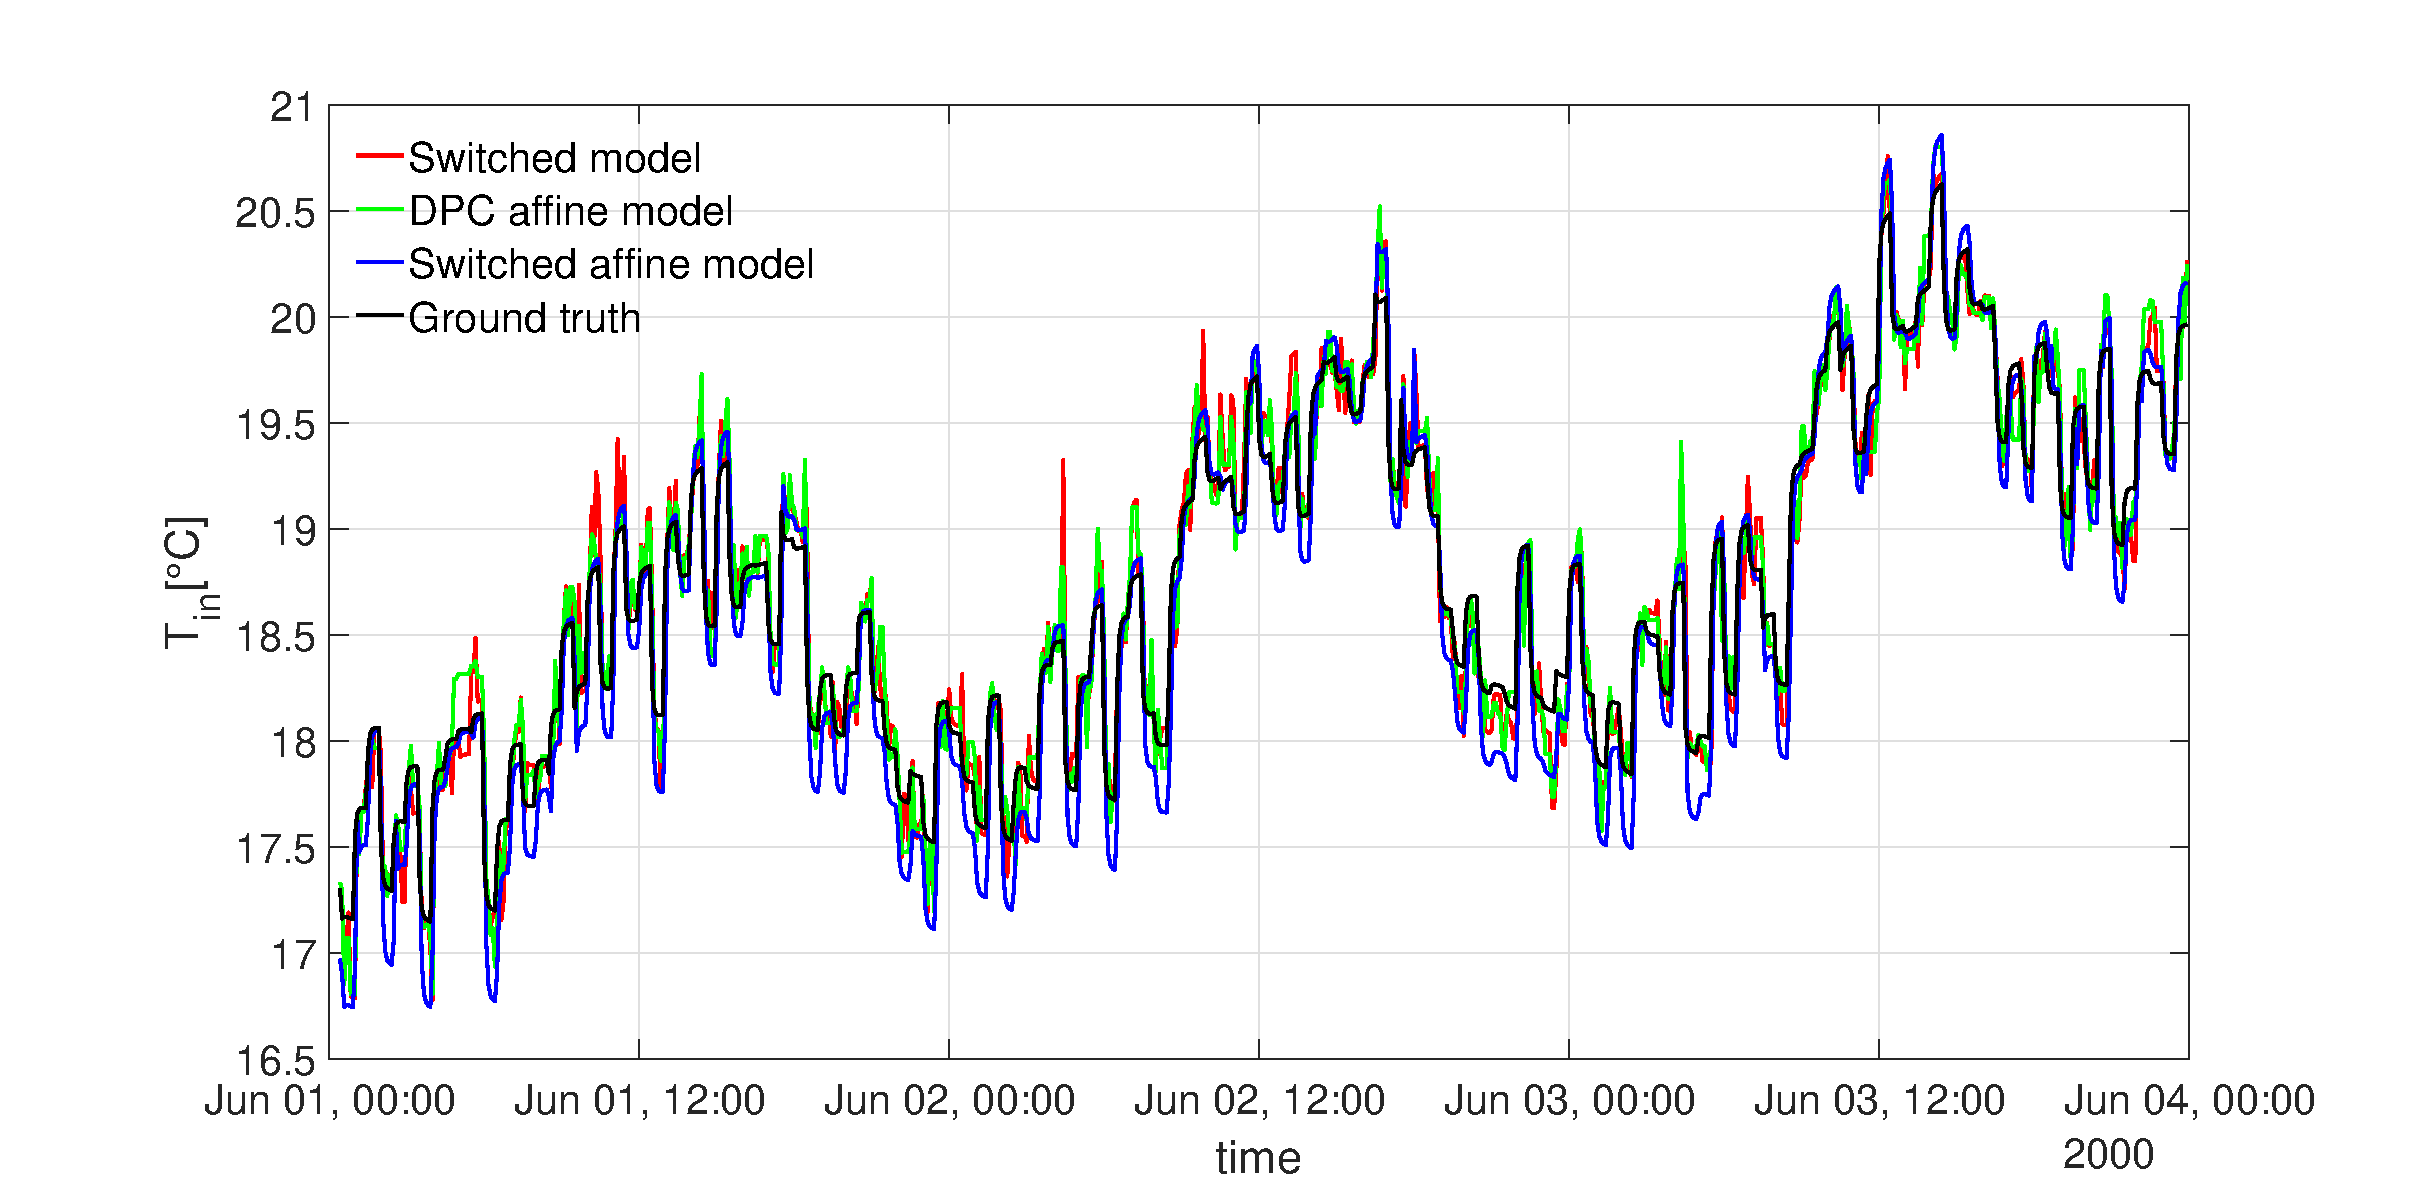
\includegraphics[width=21pc]{figures/TemperatureTesting.eps}
	\caption{Prediction accuracy along the day.}
	\label{figTesting}
\end{figure}
\begin{table}[t!]
	\begin{center}
		\caption{Comparison of the optimal solutions, provided by the DPC and the MPC with switched and switched affine models, with the optimum.}
		\label{tabComparison}
		\begin{tabular}{lcccc}
			\toprule
			Algorithm & $\mathsf{NRMSE_{x}}$ & $\mathsf{RMSE_{x}}$ & $\mathsf{NRMSE_{u}}$ & $\mathsf{RMSE_{u}}$  \\    
			\midrule
			MPC       & $0.0266$             & $0.4794$ 		   & $0$      			  & $0$      			 \\
			DPC-RT    & $0.0310$             & $0.5577$ 		   & $0.0926$ 			  & $106.96$ 			 \\
			MPC-S     & $0.0308$             & $0.5536$ 		   & $0.0506$ 			  & $58.42$  			 \\
			MPC-SA    & $0.0294$             & $0.5285$ 		   & $0.0550$ 			  & $63.59$  			 \\
			\bottomrule
		\end{tabular}
	\end{center}
\end{table}
\begin{figure}[h!]
\subfigure[Optimal control inputs.]{
\label{figInputs}
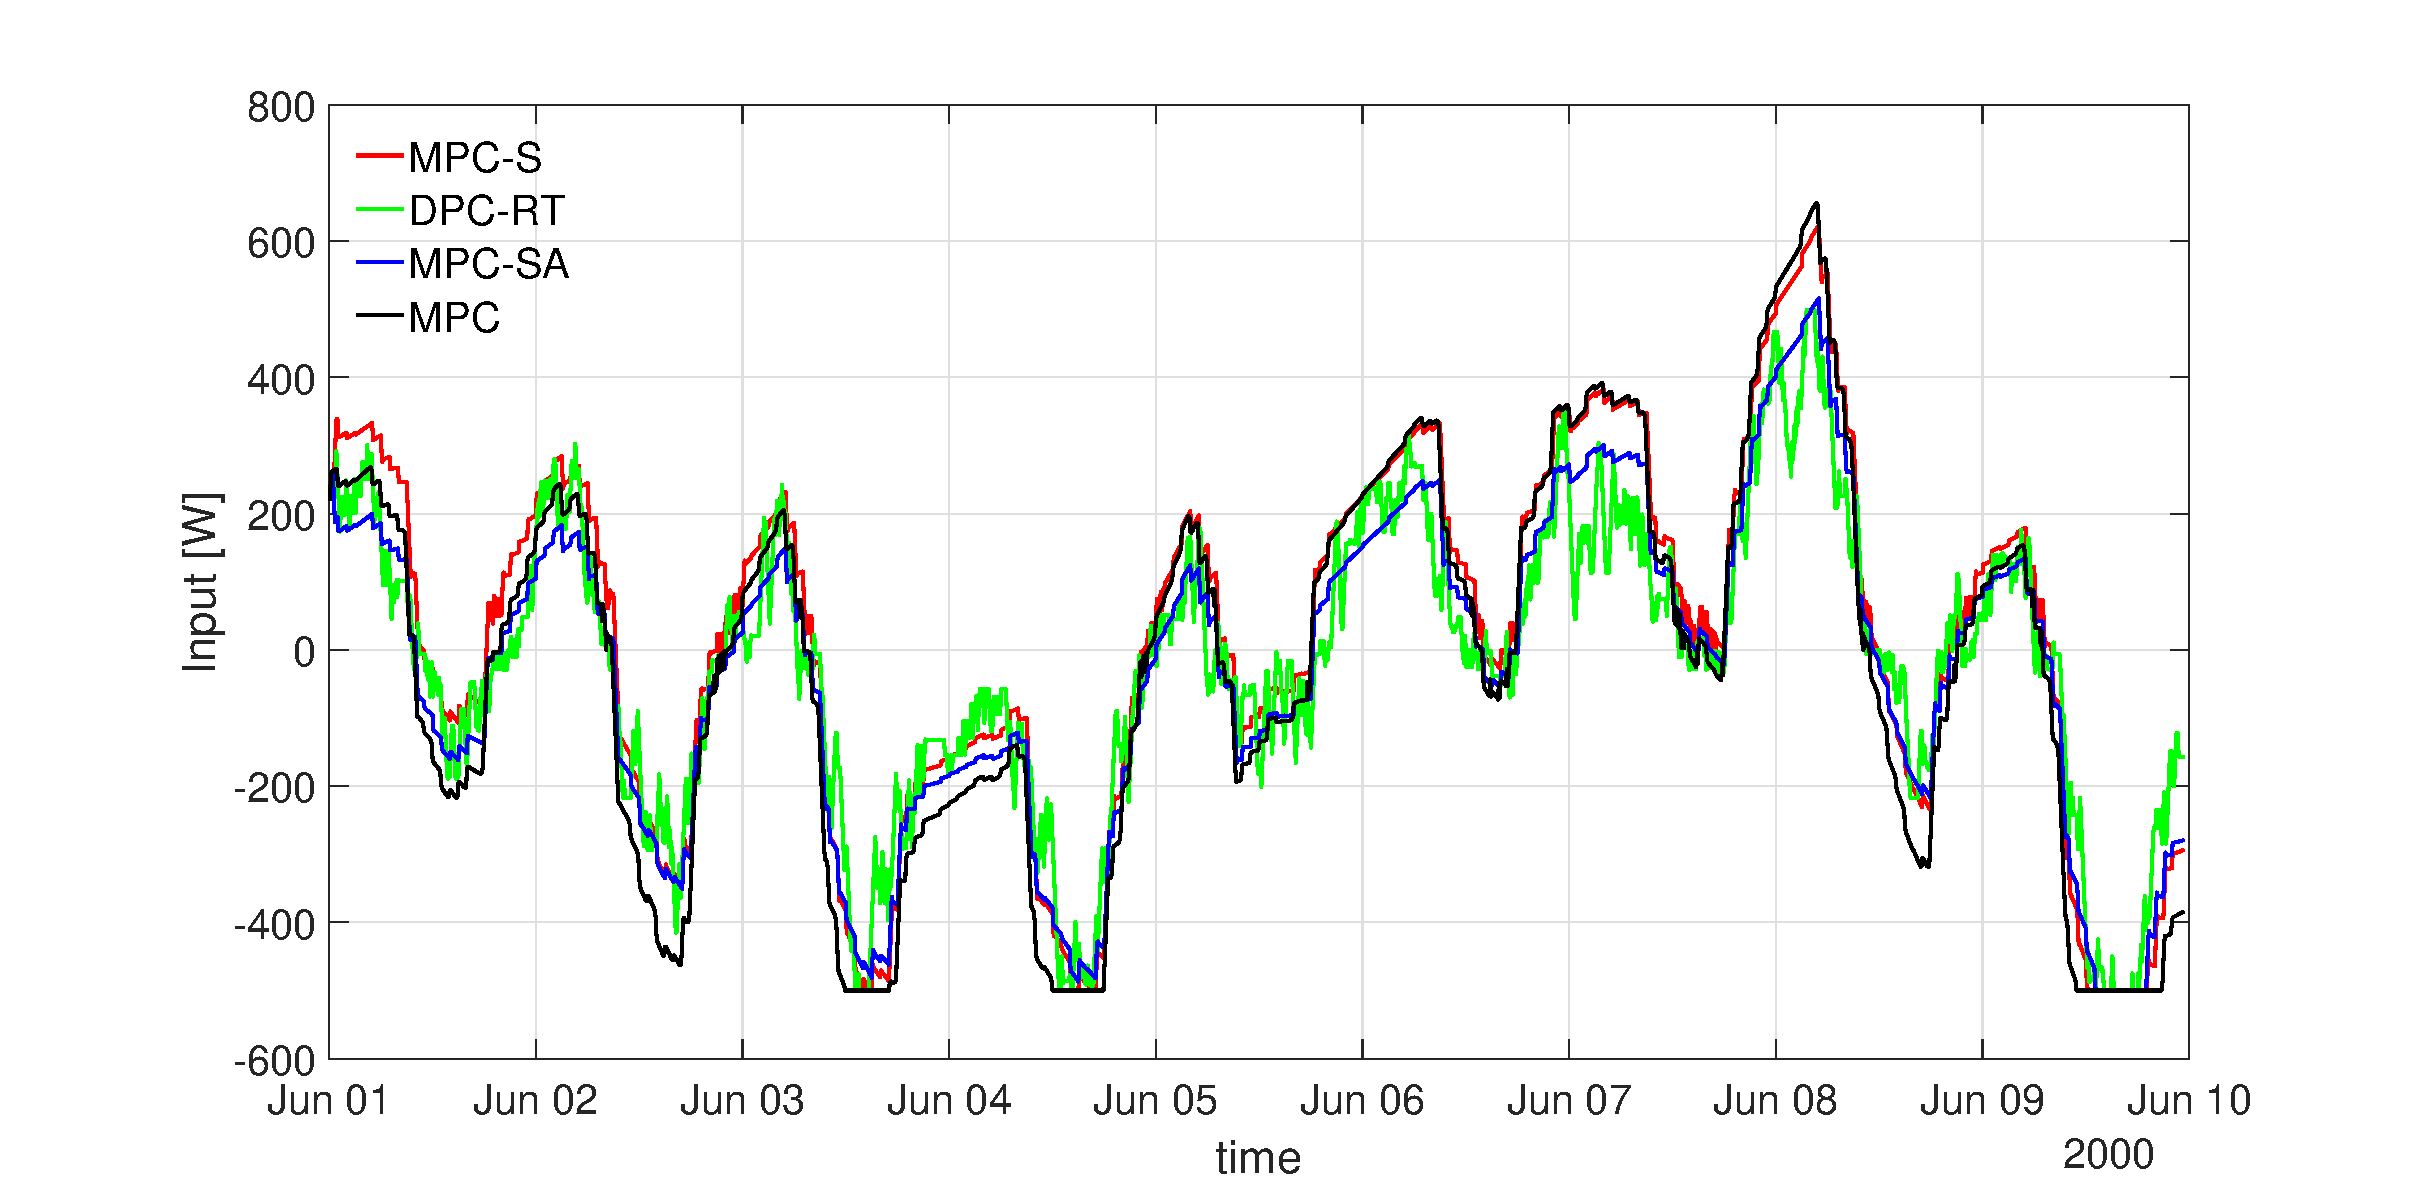
\includegraphics[width=21pc]{figures/Inputs10days.eps}}
\subfigure[Controlled temperature.]{
\label{figStates}
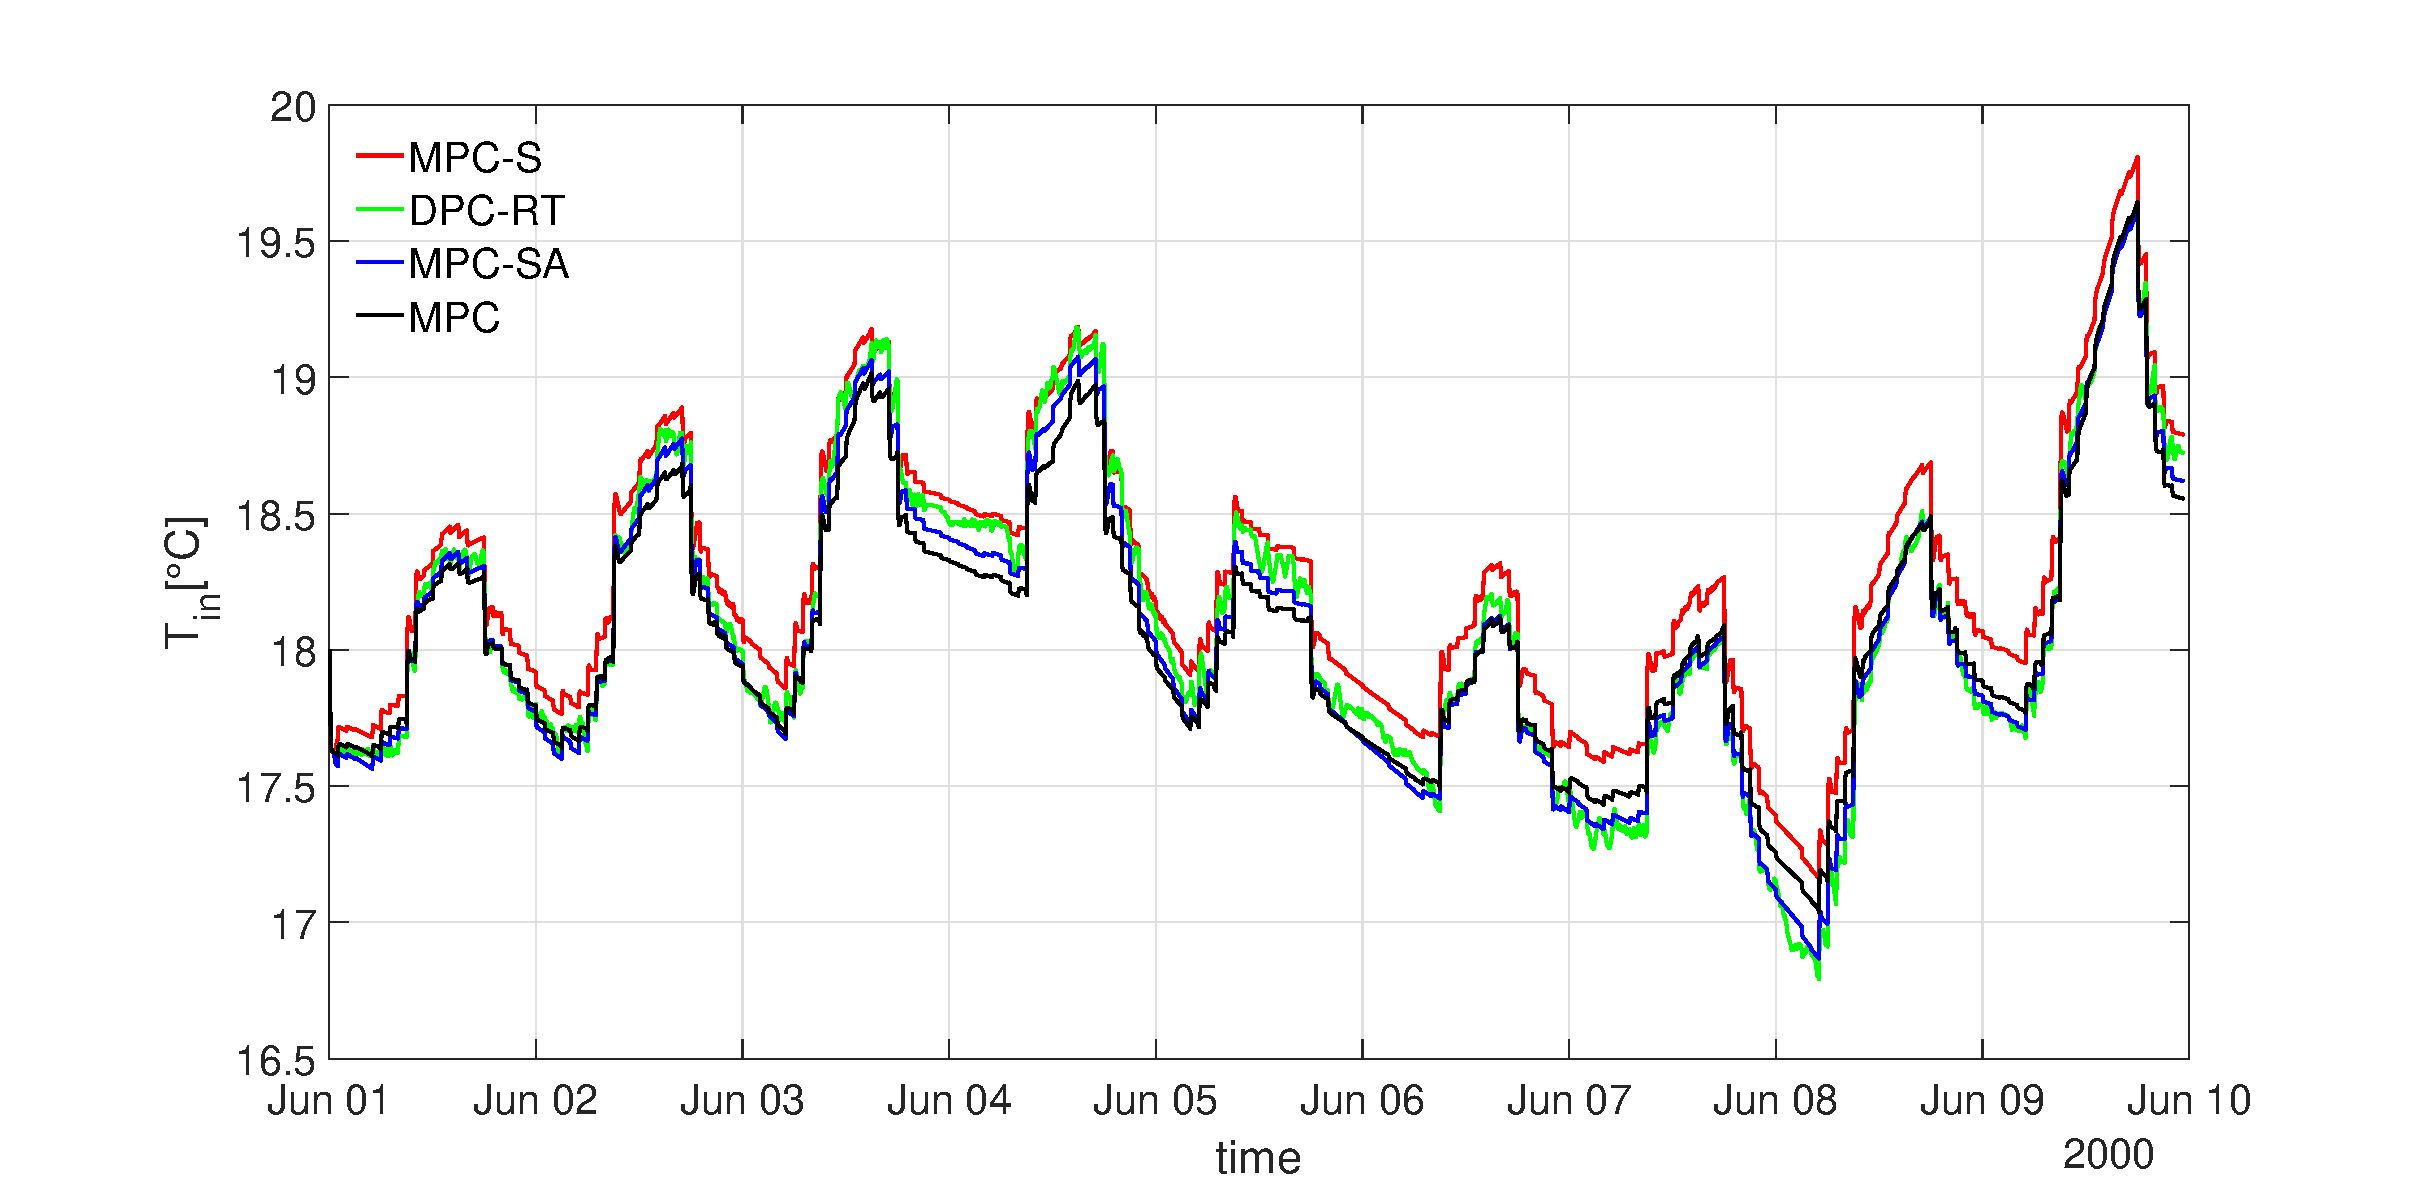
\includegraphics[width=21pc]{figures/Temperatures10days.eps}}
\subfigure[Cumulative cost function.]{
\label{figCumObjCost}
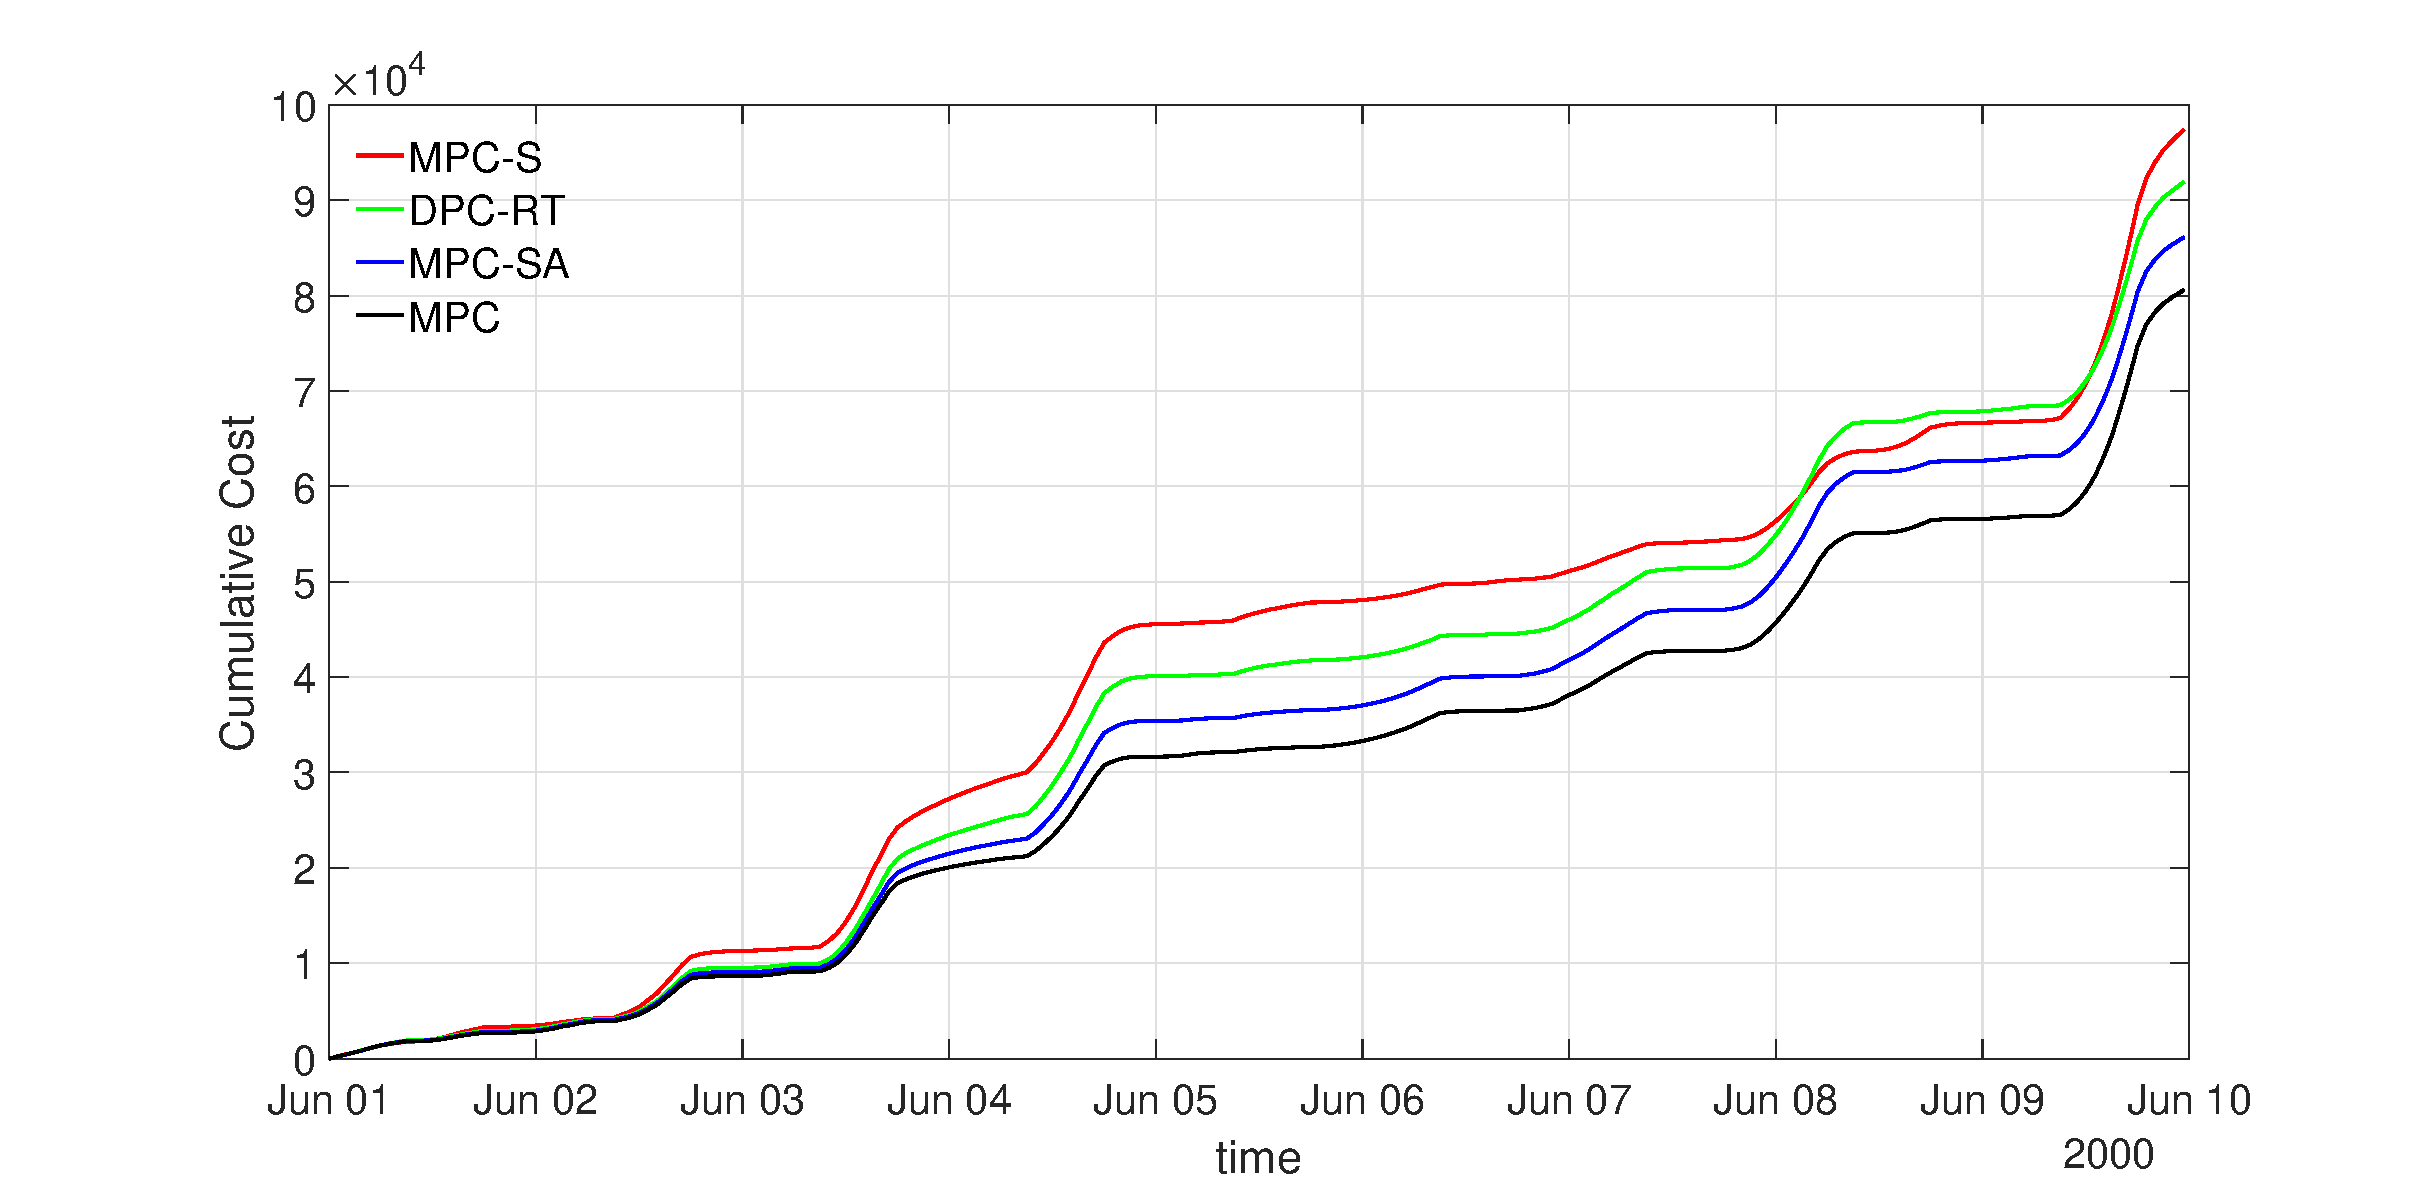
\includegraphics[width=21pc]{figures/CumulativeCost10days.eps}}
\caption{Comparison of optimal performance obtained with MPC, DPC-RT, MPC-S and MPC-SA on the period June $1^{st}$ - June $10^{th},\ 2000$.}
\label{figDPCComparisonResults}
\end{figure}

%==============================================================================================================
%==============================================================================================================

\section{CONCLUSIONS AND FUTURE WORK}\label{secConclusion}
In this paper we provide a methodology to construct a data-driven state-space switched affine model of a system from historical data, using regression trees. We setup an MPC problem and compare the performance of our control strategy against DPC, a predictive control methodology based on regression trees that uses static models to predict system's behavior. The comparison is done on DPC native case study, i.e. temperature control in a room and energy minimization. Results show that our strategy outperforms DPC in terms of optimal cost minimization.

In future work we want to extend this approach considering random forest algorithm and apply it to a problem where stability is an issue, i.e. frequency control in a microgrid. Another direction is to use this approach to improve an existing modeling by correcting the error approximation using data.

\bibliographystyle{ifacconf}
\bibliography{BAS}


\end{document}
